\documentclass[a4paper, 12pt]{article}
% math symbols
\usepackage{amssymb}
\usepackage{amsmath}
\usepackage{mathrsfs}
\usepackage{physsummer}


\usepackage{enumitem}
\usepackage[margin = 2cm]{geometry}

\tolerance = 1000
\emergencystretch = 0.74cm



\pagestyle{empty}
\parindent = 0mm

\begin{document}

\begin{center}
  \Large{\textbf{10 класс, общее тестирование по механике.}\\
  \textit{?? сентября 2015.}}
\end{center}

\begin{center}
  \Large{\textbf{Вопросы.}} \\ \large Напишите букву, соответствующую
  правильному ответу. \\ Приводить пояснения не требуется. \\
  Везде, где необходимо, считайте $g = 10\mbox{ м/с}^2$. 
\end{center}

\task{ Камень бросают под углом 45$^{\circ}$ к горизонту на расстояние
80 м. С какой скоростью камень упал на землю? А) 7 м/с. Б) 14 м/с. В)
21 м/с. Г) 28 м/с. Д) 35 м/с. Е) Среди ответов нет правильного. }

\task{ При равномерном движении автомобиля по окружности силой,
  сообщающей ему центростремительное ускорение, является ... А) Сила
  тяжести. Б) Сила реакции опоры. В) Сила трения. Г) Среди
  перечисленных ответов нет правильного. }

\task{ Сила тяги, действующая на автомобиль массой 1000 кг, при его
  равномерном движении по прямой, равна 3000 Н. Чему равна сила
  сопротивления, возникающая при движении автомобиля? А) 0. Б) 3000
  Н. В) 7000 Н. Г) 1000 Н. Д) 13000 Н. }

\task{ На наклонной плоскости с углом $\alpha$ к горизонту неподвижно
  лежит брусок. Как направлена сила, действующая на брусок со стороны
  наклонной плоскости? А) Горизонтально. Б) Вверх вдоль наклонной
  плоскости. В) Вверх перпендикулярно наклонной плоскости. Г)
  Вертикально вверх. Д) Сила равна нулю. }

\taskpic{ Чему равна равнодействующая всех сил, действующих на тело
  массой 5 кг, если график изменения его скорости с течением времени
  представлен на рисунке? А) 5 Н. Б) 10 Н. В) 15 Н. Г) 20 Н. Д) 25
  Н. }
{
  \begin{tikzpicture}
    \draw[thick,->] (0,0) node[below] {0} -- (0,3) node[right] {\small
      $v$, м/с};
    \draw[thick,->] (0,0) -- (3,0) node[above] {\small $t$, с};
    \draw (0,0.5) node[left] {5} -- ++ (2.5,0);
    \draw (0,1) node[left] {10} -- ++ (2.5,0);
    \draw (0,1.5) node[left] {15} -- ++ (2.5,0); 
    \draw (0,2) node[left] {20} -- ++ (2.5,0);
    %
    \draw (0.5,0) node[below] {1} -- ++(0,2);
    \draw (1,0) node[below] {2} -- ++(0,2); 
    \draw (1.5,0) node[below] {3} -- ++(0,2); 
    \draw (2,0) node[below] {4} -- ++(0,2);
    \draw (2.5,0) node[below] {5} -- ++(0,2);
    %
    \draw[very thick] (0,0) -- ++(45:3cm); 
  \end{tikzpicture}
}

\task{ Два тела одновременно брошены вниз из одной точки с разными
  скоростями $V_2>V_1$. Как изменяется расстояние между телами? А)
  Остаётся неизменным. Б) Равномерно увеличивается. В) Равномерно
  уменьшается. Г) Второе тело относительно первого движется
  равнозамедленно. Д) Второе тело относительно первого движется
  равноускоренно. }

\task{ Тело движется прямолинейно. Уравнение движения тела имеет вид:
  $x = -16 - 12t + 3t^2$. Каков характер движения тела в момент
  времени $t=3$? А) Движение равноускоренное. Б) Движение
  равнозамедленное. В) Ускорение тела равно 0. Г) Скорость тела равна
  0. Д) Ответ не однозначен. }

\taskpic{ Тело движется с постоянной по модулю скоростью по
  траектории, изображённой на рисунке. На каком участке траектории
  тело имеет максимальное центростремительное ускорение? А) 1-2. Б)
  2-3. В) 3-4. Г) 4-5. Д) На всех участках ускорение одинаково. }
{
  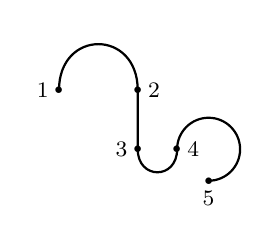
\begin{tikzpicture}
    \tikzset{point/.style={insert path={ node[scale=2.5*sqrt(\pgflinewidth)]{.} }}}
    \draw[thick] (0,0) node[point,left] {\footnotesize{1}}
    to[out=90,in=90,looseness=2] (1,0) 
    node[point,right] {\footnotesize{2}}  -- (1,-0.75)
    node[point,left] {\footnotesize{3}} 
    to[out=270,in=270,looseness=2] (1.5,-0.75) node[point,right]
    {\footnotesize{4}}; 
    \draw[thick] (1.5,-0.75) arc (180:-90:0.4cm) node[point,below]
    {\footnotesize{5}};
  \end{tikzpicture}
}

\begin{center}
  \textit{(продолжение на обороте)}
\end{center}

\task{ Шар массой $M$ движется вправо со скоростью $V$ и налетает на
  второй шар вдвое большей массы, движущийся навстречу со скоростью
  вдвое меньшей. Как будут двигаться шары после абсолютно упругого
  удара? А) Оба вправо. Б) Оба влево. В) Первый остановится, второй
  влево. Г) Первый влево, второй вправо. Д) Оба остановятся. }

\task{ Замкнутая система, в которой действуют консервативные силы и
  силы трения, перешла из состояния с кинетической энергией 100 Дж и
  потенциальной энергией 100 Дж в состояние с кинетической энергией
  150 Дж и потенциальной энергией 20 Дж. Определите работу сил трения
  в этом переходе. А) 30 Дж. Б) 50 Дж. В) 80 Дж. Г) $-$30 Дж. Д) Среди
  перечисленных ответов нет правильного. }

\task{ Уравнение движения материальной точки имеет вид
  $x=2-4t+t^2$. Определите импульс и кинетическую энергию точки массой
  1 кг через 2 с после начала отсчёта времени. А) $-$4 кг $\cdot$ м/с, 8
  Дж. Б) 0 кг $\cdot$ м/с, 0 Дж. В) $-$4 кг $\cdot$ м/с, 4 Дж. Г) 6 кг
  $\cdot$ м/с, 3 Дж. Д) Среди перечисленных ответов нет правильного.   }

\taskpic{ Зависимость потенциальной энергии $W$ взаимодействия двух
  частиц от расстояния $r$ между ними показана на рисунке. При каких
  расстояния между частицами они находятся в состоянии устойчивого или
  неустойчивого равновесия? А) 1 и 3 --- устойчивое. Б) 1 и 3 ---
  неустойчивое, 5 --- устойчивое. В) 2 --- устойчивое, 4 ---
  неустойчивое. Г) 2 --- неустойчивое, 4 --- устойчивое. Д) Среди
  перечисленных ответов нет правильного. }
{
  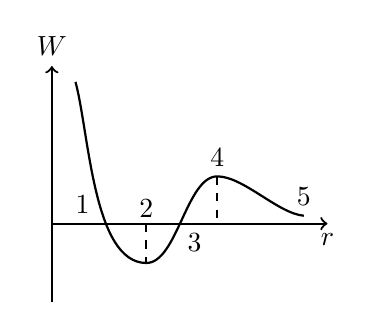
\begin{tikzpicture}
    \draw[thick,->] (0,0) -- (3.5,0) node[below] {$r$};
    \draw[thick,->] (0,-1) -- (0,2) node[above] {$W$};
    \draw[thick] (0.3,1.8) to[out=285,in=180,looseness=0.7] (1.2,-0.5)
    node[above=0.45cm] {2}
    to[out=0,in=180,looseness=0.7] (2.1,0.6) node[above] {4}
    to[out=0,in=175,looseness=0.7] 
    (3.2,0.1) node[above] {5};
    \draw[thick,dashed] (1.2,0) -- (1.2,-0.5);
    \draw[thick,dashed] (2.1,0.6) -- (2.1,0);
    \draw (0.6,0) node[above left] {1};
    \draw (1.6,0) node[below right] {3}; 
  \end{tikzpicture}
}

\setcounter{notask}{1}

\begin{center}
  \Large{\textbf{Задачи.}} \\ \large Напишите полное решение. 
\end{center}

\task{ Пушка стреляет со скоростью 100 м/с под углом к горизонту не
  менее 30$^{\circ}$. Может ли снаряд поразить цель на расстоянии 500
  м по горизонтали, не поднимаясь выше 375 м над точкой выстрела?
  Сопротивление воздуха мало. }
% Зильберман

\task{ Тело массы $m$ стоит на горизонтальной плоскости. К телу
  приложена сила $F$ под углом $\alpha$ к горизонту. При каких
  значениях коэффициента трения $\mu$ между телом и плоскостью оно
  останется неподвижным? }
% Манида

\task{ На горизонтальном гладком столе покоится клин массы $M$ с углом
  $\alpha$ при основании. На него наезжает со скоростью $V_0$
  маленькое тело массы $m$ и начинает подниматься вверх по клину (у
  основания клина сделан плавный <<въезд>>). При какой высоте клина
  $H$ маленькое тело поднимется по нему на самый верх? }
% Зильберман


\end{document}


%%% Local Variables: 
%%% mode: latex
%%% TeX-engine:xetex
%%% TeX-PDF-mode: t
%%% End:
